\scanpage{22}
\noindent\begin{minipage}[t]{.30\linewidth}
\figure{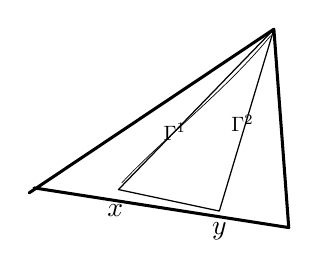
\begin{tikzpicture}[x=.021cm,y=-.021cm,line join=round,line cap=round]
\draw[line width=1.1pt] (0,102)--(148,3)--(157,123)--(3,99);
\draw[line width=.45pt] (148,3)--(54,100)--(115,113)--cycle;
\draw[line width=.25pt] (56,96)..controls (79,71) and (119,40)..(146,7);
\node[below] at (52,103) {$x$};
\node[below] at (115,114) {$y$};
\node[inner sep=0pt,scale=.75] at (88,65) {$\Gamma^{1}$};
\node[inner sep=0pt,scale=.75] at (129,60) {$\Gamma^{2}$};
\end{tikzpicture}}
\end{minipage}\hfill
\begin{minipage}[t]{.67\linewidth}
\small
\[
\left\{\begin{aligned}
\Gamma^{1}_{xy}\cap\Gamma^{2}_{xy}&=\{x,y\}\\
\Gamma^{1}_{x,y}\cup\Gamma^{2}_{x,y}&=\Gamma\\
S'(\Gamma^{1}_{\unsure{x|xx}y})\cup S'(\Gamma^{2}_{xy})&=S(\Gamma)\setminus\{x,y\}\unsure{\cap S(\Gamma|S(\Gamma}
\end{aligned}\right.
\]
\uline{NB} Ce n'est pas le \uline{couple} $(\Gamma^{1}_{xy},\Gamma^{2}_{xy})$ qui est déterminé de façon unique mais l'\uline{ens} $\{\Gamma^{1}_{xy},\Gamma^{2}_{x,y}\}$
\end{minipage}

a) op. de \unsure{rajouter|rajout de} \unsure{sommet|sommets}

b) op. de division d'un polygone (par 2 \unsure{sommets|sommet} distincts) en deux lignes polygonales (op. inverse : recollement de 2 lignes polygonales ayant $=$ extrémités).

\figure{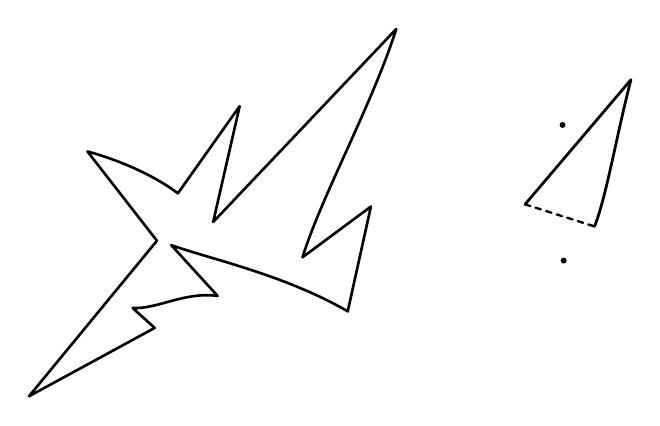
\begin{tikzpicture}[x=.014cm,y=-.014cm,line join=round,line cap=round]
\draw[line width=.95pt] (53,112)..controls (89,122) and (118,137)..(135,150)--(191,71)--(167,176)--(333,1)..controls (311,70) and (265,153)..(248,208)--(310,162)--(289,257)..controls (232,224) and (166,210)..(129,197)--(171,243)..controls (141,239) and (117,255)..(94,254)--(114,272)--(0,334)--(116,193)--cycle;
\begin{scope}[xshift=6.3cm]
\draw[line width=1pt] (0,160)--(96,47)..controls (83,97) and (74,152)..(63,180);
\draw[dash pattern=on 2pt off 2pt,line width=.85pt] (0,160)--(63,180);
\fill (34,88) circle[radius=2.7];
\fill (35,211) circle[radius=2.7];
\end{scope}
\end{tikzpicture}}
% archive sheet number: 21
